\sectionframe{Scenario method}
\begin{frame}
 \frametitle{Example: Relieve Ethiopia}
 Long term warehouse capacity: 8 houses
 \begin{block}{Warehouse demand:}\scriptsize
  \centering
  \begin{tabularx}{\textwidth}{l*{4}{>{\centering\arraybackslash}X}}
   \toprule
      &  Scenario I &  Scenario II &  Scenario III &  Scenario IV\\
     Resource & (30\%) & (30\%) & (25\%) & (15\%)\\
   \midrule
    Food 	& 4 & 2 & 3 & 4\\
    Dringking water & 3 & 5 & 3 & 5\\
    Medication & 3 & 3 & 1 & 4\\
   \bottomrule
  \end{tabularx}
 \end{block}
 \begin{block}{Short term warehouse costs}
  \begin{itemize}
    \item 3500\$ for a food warehouse
    \item 1600\$ for a drinking water warehouse
    \item 5200\$ for a medication warehouse
  \end{itemize}
 \end{block}
\end{frame}

\begin{frame}
 \frametitle{Two stage stochastic optimization}
 \begin{figure}
  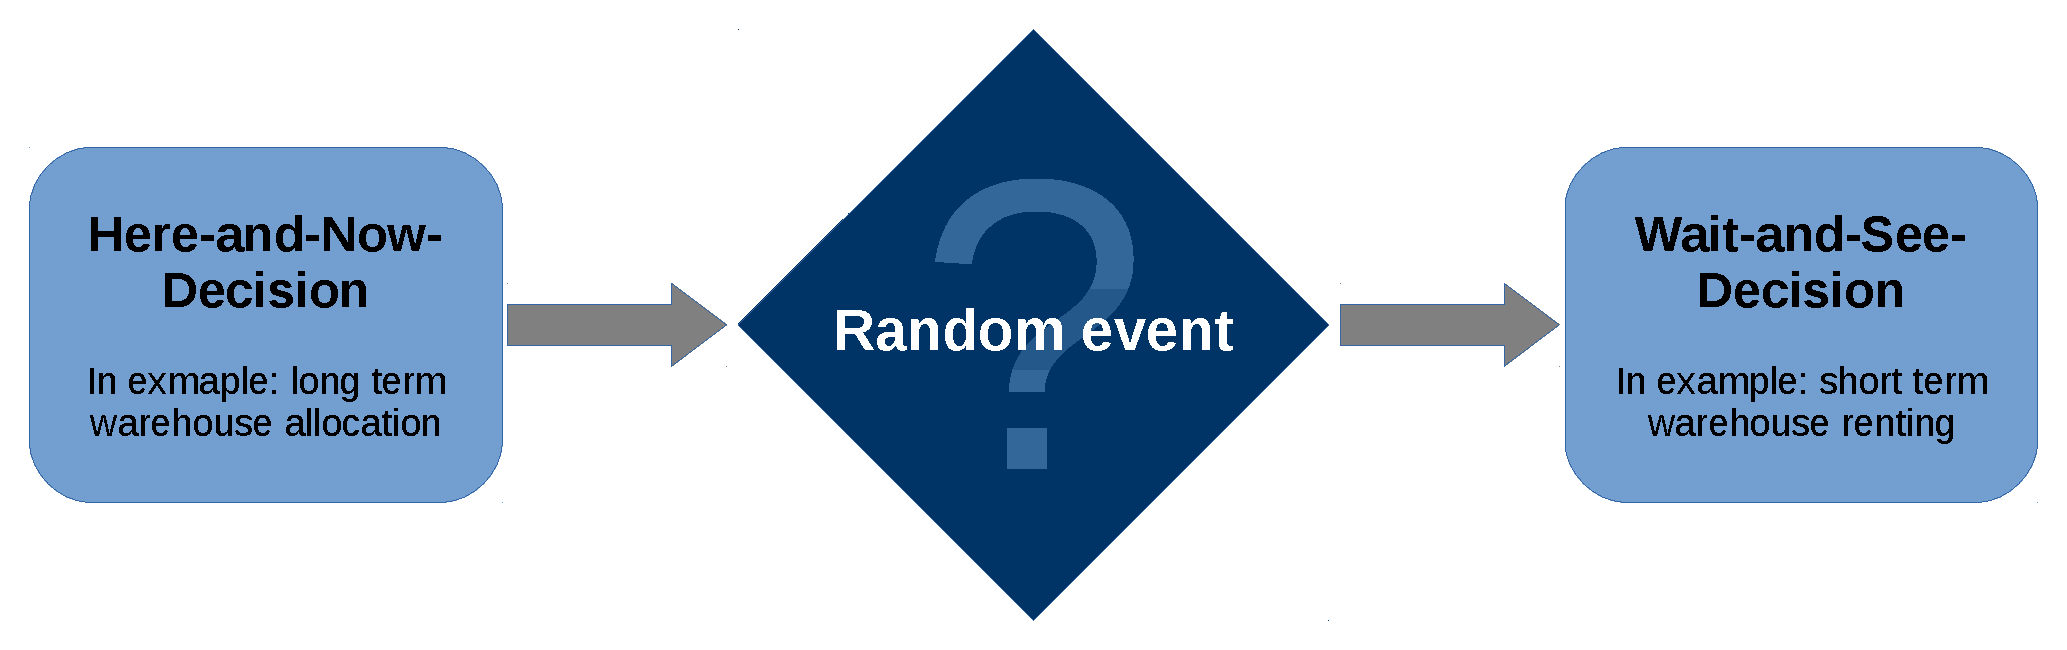
\includegraphics[width=\linewidth]{Bilder/Scenariomethode}
 \end{figure}
 \begin{block}{Scenario method}
  \begin{itemize}
   \item Special case of two stage stochastic optimization
   \item Random event = occurance of one out of a finite number of scenarios 
   \item Stochastic objective function often replaced by expected value
  \end{itemize}
 \end{block}
\end{frame}

\begin{frame}
 \frametitle{Equivalent deterministic model using scenario method}
 \begin{itemize}
  \item Index set~$I$ of scenarios
  \item Parameter~$p_i$: probability of scenario~$i\in I$
  \item Scenario independent parameters and here-and-now-decision-variables have no scenario index
  \item Scenario dependent parameters and wait-and-see-decision-variables have a scenario index
  \item With a finite number of scenarios, the expected value becomes a convex combination and is therefore linear
 \end{itemize}
\end{frame}

\begin{frame}
 \frametitle{Model: stochastic resource planning}
 \footnotesize
 \begin{tabularx}{\linewidth}{lL}
  \multicolumn{2}{l}{\textbf{Index sets}:}\\
     $I$ & set of scenarios\\
     $R$ & set of resources\\
  \multicolumn{2}{l}{\textbf{Parameters}:}\\
     $p_i$ & probability of scenario~$i\in I$\\
     $c_r$ & cost for additional short term capacity of resource~$r\in R$\\
     $d_{ri}$ & demand of resource~$r\in R$ in scenario~$i\in I$ \\
     $k$ & capacity for long term resource allocation\\
  \multicolumn{2}{l}{\textbf{Decision variables}:}\\
     $x_{r}$ & long term capacity allocated to resource~$r\in R$\\
     $y_{ri}$ & short term capacity bought for resource~$r\in R$ in scenario~$i\in I$\\[1ex]
  \multicolumn{2}{l}{\textbf{Model description}:}\\[1ex]
  \multicolumn{2}{l}{
      $
      \begin{array}{rllr}
	\min & \multicolumn{3}{l}{
		  \displaystyle\sum_{i\in I}p_i\cdot\left(\sum_{r\in R}c_r\cdot y_{ri}\right)
		}\\[3ex]
	s.t. & \displaystyle\sum_{r\in R} x_{r} \leq k &  & \mathrm{(I)}\\
	      & x_r + y_{ri} \geq d_{ri}  & \quad\forall r\in R, i\in I  & \mathrm{(II)}\\[.8ex]
	      & x_r, y_{ri} \in \mathbb{Z}^+ & \quad\forall r\in R, i\in I &\\
      \end{array}
      $ 
  }\\[1ex]
 \end{tabularx}
\end{frame}



